% Number 800
% CAPMG Units 
% x graph -find v, a
% JG

% Watermark
\AddToShipoutPicture*{\BackgroundPic}

\addtocounter {ProbNum} {1}

%\begin{floatingfigure}[r]{.44\textwidth}
%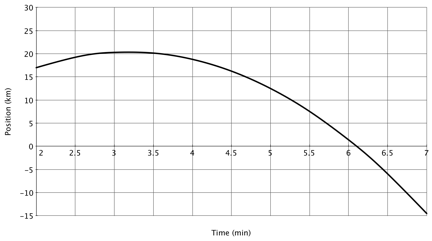
\includegraphics[scale=.5]{/Users/jgates/desktop/latex/pics/xgraph2}
%\end{floatingfigure}
 
{\bf \Large{\arabic{ProbNum}}} Use the graph to determine the object's initial velocity and its acceleration, using graphical methods. Draw any additional graphs that you need for your solution below.\bigskip

\begin{center}
 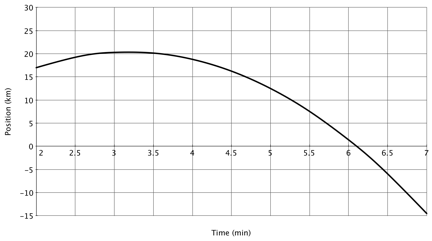
\includegraphics[scale=1]{/Users/jgates/desktop/latex/pics/xgraph2}
\end{center}

\vfill
\newpage